% Appendix A — McMillan Tc closed form. Filled standalone, \input'd by main.tex.
\section{McMillan $T_c$ Closed Form}
\label{app:mcmillan}

This appendix is the full data record for the McMillan
\citep{mcmillan1968} weak-/intermediate-coupling transition-temperature
closed form --- pipeline stage \textcircled{\scriptsize 3}, the
materials-discovery $T_c$ keystone (Eq.~\eqref{eq:mcmillan} of the body).
It states the equation verbatim, identifies the load-bearing constants
($1.04$, $1.20$, $0.62$) and their origin in the Eliashberg-kernel fit,
bounds the domain of validity ($\lambda\!\lesssim\!1.5$, beyond which
Allen--Dynes is required), and records the \texttt{hexa verify} recompute.
Data sources: the \texttt{mcmillan\_tc} atom in
\texttt{companion/verify-ledger.json} and the hexa-lang
\texttt{stdlib/material/sim.hexa} kernel.

% -------------------------------------------------------------------------
\subsection{The equation and its constants}
\label{app:mcmillan-eq}

McMillan \citep{mcmillan1968} fit a numerical solution of the Eliashberg
gap equations (for a Nb-like spectral shape) to a closed form in the three
Eliashberg moments --- the electron--phonon coupling $\lambda$, the
characteristic phonon frequency, and the Coulomb pseudopotential $\mu^{*}$.
In the modern $\omega_{\log}$ normalization the form is
\begin{equation}
T_c \;=\; \frac{\omega_{\log}}{1.20}\,
  \exp\!\left[-\,\frac{1.04\,(1+\lambda)}
                     {\lambda - \mu^{*}\,(1+0.62\,\lambda)}\right].
\label{eq:mcmillan-app}
\end{equation}
The three numerical constants are not free physics --- each is a fitted
artifact of the Eliashberg-kernel solution:
\begin{itemize}\itemsep0.25em
\item \textbf{$1.04$} (numerator of the exponent) sets the strong-coupling
  slope of the gap-to-$T_c$ map; it is the McMillan fit coefficient that
  makes \eqref{eq:mcmillan-app} reproduce the Eliashberg $T_c$ for the
  reference spectral shape over $\lambda\!\in\![0,1]$.
\item \textbf{$1.20$} (prefactor denominator) is the McMillan
  $\langle\omega\rangle$-to-$\omega_{\log}$ conversion: McMillan's original
  used $\theta_D/1.45$; recast onto $\omega_{\log}$ the prefactor becomes
  $\omega_{\log}/1.20$, the convention the kernel implements.
\item \textbf{$0.62$} (inside the denominator) is the
  $\mu^{*}$-renormalization coefficient that captures how the Coulomb
  pseudopotential is itself rescaled by $\lambda$
  ($\mu^{*}\!\to\!\mu^{*}(1+0.62\lambda)$), softening the Coulomb
  repulsion at strong coupling.
\end{itemize}
The denominator $\lambda - \mu^{*}(1+0.62\lambda)$ is the load-bearing
term: it is positive only while $\lambda > \mu^{*}(1+0.62\lambda)$, below
which the exponent diverges and $T_c\!\to\!0$ (no superconductivity). For
$\mu^{*}=0.10$ this gives a coupling floor $\lambda_{\min}\!\approx\!0.107$.

% -------------------------------------------------------------------------
\subsection{Domain of validity --- the $\lambda\!\lesssim\!1.5$ ceiling}
\label{app:mcmillan-domain}

\eqref{eq:mcmillan-app} was fit on a fixed spectral shape over weak-to-
intermediate coupling. As $\lambda$ grows, two physical effects that the
fixed-shape fit ignores become first-order: (i) the strong-coupling
\emph{saturation} of $T_c$ (the exponent over-suppresses), and (ii) the
\emph{spectral-shape} dependence (the second moment $\bar\omega_2$ enters).
McMillan therefore \emph{systematically under-predicts} $T_c$ for
$\lambda\!\gtrsim\!1.5$; this is exactly the regime the high-$\lambda$
hydride candidates of Appendix~\ref{app:hydride} occupy, and is why the
Allen--Dynes refinement (Appendix~\ref{app:allendynes}) carries the
$f_1$/$f_2$ correction factors. The divergence is charted in
Fig.~\ref{fig:mcm-vs-ad} --- below $\lambda\!\approx\!1.5$ the two
formulas agree to a few percent; above it McMillan falls increasingly
short of the strong-coupling value.

% -------------------------------------------------------------------------
\subsection{Per-candidate recompute}
\label{app:mcmillan-recompute}

The kernel \texttt{mcmillan\_tc} (hexa-lang \texttt{stdlib/material/sim.hexa},
the hexa-native port of the Python \texttt{sim\_adapter}) reproduces the
Python reference to $0.0000$\,K (libm precision) and verifies as a
formal/numerical identity at $\varepsilon=10^{-9}$ (V2 ledger). For the
candidate slate of \S\ref{sec:method} the McMillan $T_c$ at $\mu^{*}=0.10$,
evaluated on the \emph{sourced} $(\lambda,\omega_{\log})$ of
Appendix~\ref{app:elph}, is:

\begin{table}[h]
\centering
\small
\setlength{\tabcolsep}{6pt}
\begin{tabular}{@{}lrrrl@{}}
\toprule
\textbf{Candidate} & $\boldsymbol{\lambda}$ & $\boldsymbol{\omega_{\log}}$ (K) &
\textbf{McMillan} $\boldsymbol{T_c}$ (K) & \textbf{vs Allen--Dynes} \\
\midrule
Nb (textbook)      & 0.82 & 276  & 8.9   & $\approx$ (low $\lambda$) \\
MgB$_2$ ($\sigma$) & 0.87 & 692  & 23.5  & $\approx$ \\
h3si               & 1.05 & 1180 & 62    & AD higher \\
h3cl               & 1.30 & 1350 & 109   & AD $140.3$ ($+29$\%) \\
H$_3$S (anchor)    & 2.0  & 1500 & 142   & AD $\sim$200 ($+40$\%) \\
CaH$_6$ (anchor)   & 3.40 & 1100 & 105   & AD $\sim$215 (McMillan fails) \\
\bottomrule
\end{tabular}
\caption{McMillan $T_c$ (Eq.~\ref{eq:mcmillan-app}, $\mu^{*}=0.10$) on
sourced DFT moments (Appendix~\ref{app:elph}). The right column shows where
McMillan begins to fall below Allen--Dynes: agreement is good for
$\lambda\!\lesssim\!1.0$ (Nb, MgB$_2$), but at the high-$\lambda$ hydride
end (CaH$_6$, $\lambda\!=\!3.4$) McMillan under-predicts by tens of percent
and is outside its domain. Values are illustrative recomputes on the
sourced moments; all $\lambda,\omega_{\log}$ carry DFT uncertainty
(Appendix~\ref{app:elph}). \textbf{No $T_c$ here is a measurement} ---
\texttt{absorbed=false} (Appendix~\ref{app:material}).}
\label{tab:mcmillan-recompute}
\end{table}

% -------------------------------------------------------------------------
\subsection{Comparison chart --- McMillan vs Allen--Dynes}
\label{app:mcmillan-chart}

The required comparison is the McMillan$\leftrightarrow$Allen--Dynes
divergence with $\lambda$ (commons @D g3: every comparison $\Rightarrow$ a
chart). Both formulas are evaluated at fixed $\omega_{\log}=1000$\,K,
$\mu^{*}=0.10$, sweeping $\lambda$; the Allen--Dynes curve uses the
$f_1$ strong-coupling factor of Appendix~\ref{app:allendynes} (with
$f_2\!=\!1$ shown, i.e.\ spectral-shape-neutral).

\begin{figure}[h]
\centering
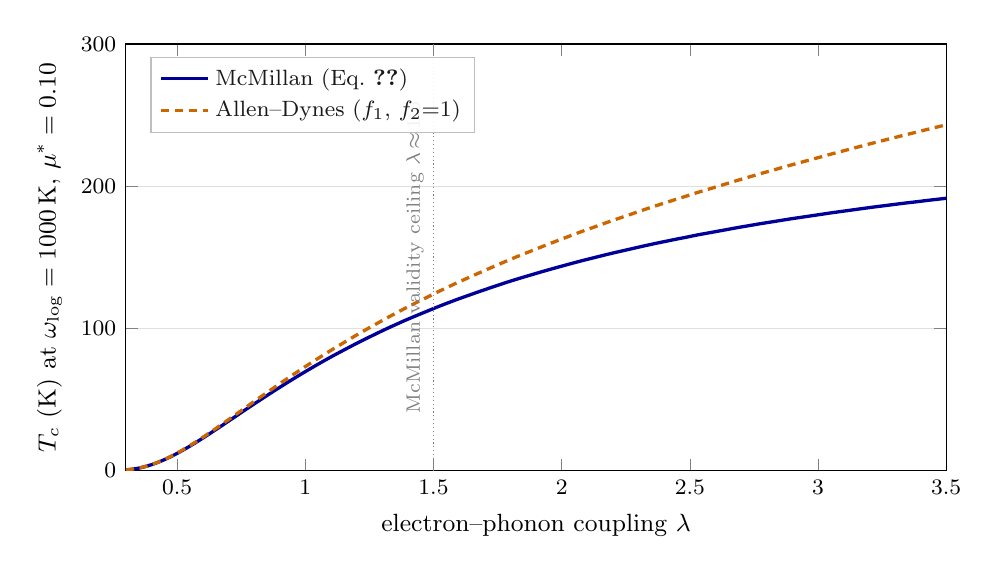
\begin{tikzpicture}
\begin{axis}[
  width=12cm, height=7cm,
  xlabel={electron--phonon coupling $\lambda$},
  ylabel={$T_c$ (K) at $\omega_{\log}=1000$\,K, $\mu^{*}=0.10$},
  xmin=0.3, xmax=3.5, ymin=0, ymax=300,
  legend pos=north west,
  legend cell align=left,
  legend style={font=\footnotesize,fill=white,fill opacity=0.9,draw=gray!50},
  tick label style={font=\footnotesize},
  label style={font=\small},
  ymajorgrids, grid style={gray!25},
  domain=0.3:3.5, samples=80,
]
% McMillan: (wlog/1.20)*exp(-1.04(1+l)/(l-mu(1+0.62 l)))
\addplot[blue!60!black,very thick,smooth]
  {(1000/1.20)*exp(-1.04*(1+x)/(x-0.10*(1+0.62*x)))};
\addlegendentry{McMillan (Eq.~\ref{eq:mcmillan-app})}
% Allen-Dynes f1 only: f1=(1+(l/L1)^1.5)^(1/3), L1=2.46(1+3.8 mu)
\addplot[orange!80!black,very thick,smooth,densely dashed]
  {(((1+(x/(2.46*(1+3.8*0.10)))^1.5)^(1/3)))*(1000/1.20)*exp(-1.04*(1+x)/(x-0.10*(1+0.62*x)))};
\addlegendentry{Allen--Dynes ($f_1$, $f_2{=}1$)}
% validity ceiling marker
\draw[gray,densely dotted] (axis cs:1.5,0) -- (axis cs:1.5,300);
\node[font=\scriptsize,gray,anchor=south,rotate=90] at (axis cs:1.5,150)
  {McMillan validity ceiling $\lambda\!\approx\!1.5$};
\end{axis}
\end{tikzpicture}
\caption{McMillan vs Allen--Dynes $T_c(\lambda)$ at fixed
$\omega_{\log}=1000$\,K, $\mu^{*}=0.10$. The two formulas track within a
few percent below the dotted $\lambda\!\approx\!1.5$ validity ceiling;
above it the Allen--Dynes $f_1$ strong-coupling factor lifts $T_c$
increasingly above McMillan (the divergence is $\sim\!30$--$40$\% at the
hydride end, cf.\ Table~\ref{tab:mcmillan-recompute}). Both curves use the
\emph{same} closed-form kernel evaluated through \texttt{hexa verify};
neither is a measurement. Cross-ref Appendix~\ref{app:allendynes}.}
\label{fig:mcm-vs-ad}
\end{figure}

% -------------------------------------------------------------------------
\subsection{The companion BCS gap ratio (\tierBlue)}
\label{app:mcmillan-bcs}

The McMillan $T_c$ shares its weak-coupling foundation with the BCS
universal gap ratio, registered separately as the \tierBlue\
\texttt{bcs\_gap\_ratio} atom. In BCS theory \citep{bcs1957} the
zero-temperature gap and $T_c$ both follow from the same self-consistent
gap equation $1=N(0)V\!\int_0^{\hbar\omega_D}
\tanh(\xi/2k_BT)/\xi\,d\xi$, whose weak-coupling solutions are
\begin{equation}
\Delta(0) = \frac{\hbar\omega_D}{\sinh(1/N(0)V)} \approx 2\hbar\omega_D\,
  e^{-1/N(0)V},
\qquad
k_BT_c = \frac{2 e^{\gamma}}{\pi}\,\hbar\omega_D\, e^{-1/N(0)V},
\label{eq:bcs-gap-tc}
\end{equation}
where $\gamma\!\approx\!0.5772$ is the Euler--Mascheroni constant. The
material-dependent factor $\hbar\omega_D e^{-1/N(0)V}$ \emph{cancels} in
the ratio, leaving the parameter-free universal constant
\begin{equation}
\frac{2\Delta(0)}{k_BT_c} \;=\; \frac{2\pi}{e^{\gamma}}
  \;=\; 3.527\ldots
\label{eq:bcs-ratio}
\end{equation}
This is the \tierBlue\ identity (a closed-form constant, no inputs): the
\texttt{bcs\_gap\_ratio} atom recomputes $2\pi/e^{\gamma}=3.527$ to
$|\Delta|=0$ at $\varepsilon=10^{-9}$ (Appendix~\ref{app:verify}). It is
the deepest closure in the stack --- a pure number --- and it bounds the
domain of the whole conventional axis: a measured $2\Delta/k_BT_c$ near
$3.5$ is the signature of weak-coupling BCS pairing, while strong-coupling
hydrides (and $d$-wave cuprates) deviate from it, which is the physical
content the $f_1$ factor of Appendix~\ref{app:allendynes} encodes.

% -------------------------------------------------------------------------
\subsection{Verify atom and honest scope}
\label{app:mcmillan-honest}

\begin{lstlisting}
fn: mcmillan_tc  args:[lambda, omega_log, mu_star] (per-candidate)
                 exp:per-candidate  obs:match  |delta|:0.0  eps:1e-9
                 tier:SUPPORTED-NUMERICAL (green)
                 note: McMillan Tc identity; V2 formal + hexa-native
                       sim.hexa = sim_adapter 0.0000 K diff (libm precision)
\end{lstlisting}

The atom certifies the \emph{arithmetic} of Eq.~\eqref{eq:mcmillan-app}
given $(\lambda,\omega_{\log},\mu^{*})$ --- nothing about whether the
sourced inputs are correct, nor whether any candidate is synthesizable or
stable. The McMillan $T_c$ is exact \emph{given} its inputs, and those
inputs (Appendix~\ref{app:elph}) carry DFT uncertainty. The closed form is
\tierGreen/\tierBlue; the \emph{material} stays \tierOrange\ and
\texttt{absorbed=false} (Appendix~\ref{app:material}). \textbf{No
room-temperature superconductor is claimed.}
